%%TODO: Label setzen\

%Dokument erstellen
\documentclass[a4paper,DIV11,bibliography=totoc,headings=normal,ngerman,headsepline,listof=totoc,parskip=half]{scrreprt}

%Benötigte Packages
\usepackage{babel} 
\usepackage[T1]{fontenc}           
\usepackage[utf8]{inputenc}  
\usepackage{graphicx}
\usepackage{amsmath}
\usepackage{lmodern}
\usepackage[printonlyused,withpage]{acronym}
\usepackage[a4paper,lmargin={2.5cm},rmargin={2.5cm},tmargin={2cm},bmargin={2.2cm}]{geometry} 
\usepackage{float}
%Library
\bibliographystyle{plain}

%Formelverzeichnis mittels KOMA-Script erstellen
\DeclareNewTOC[type=formel,name={Formel},hang=5em,listname={Formelverzeichnis}]{for}
\newcommand*{\formelentry}[1]{\addcontentsline{for}{formel}{\protect\numberline{Formel~\theequation} #1}}

%Informationen der PDF
\pdfinfo
{
/Title		(Extrapolation von Zeitreihen mit Hilfe von künstlichen neuronalen Netzen am Beispiel von Börsenprognosen)
/Subject	(Eine Anwendung im Fach Softcomputing – Teilgebiet neuronale Netze)
/Author		(Sebastian Schötteler \& Benedikt Hofrichter)
}

%Kopf- und Fußzeile
\pagestyle{headings}

\begin{document}

\subject{Seminararbeit}
\title{Extrapolation von Zeitreihen mit Hilfe von künstlichen neuronalen Netzen am Beispiel von Börsenprognosen}
\author{Sebastian Schötteler -- Matrikelnummer 2429289 \and Benedikt Hofrichter -- Matrikelnummer 2272198}
\subtitle{\bigskip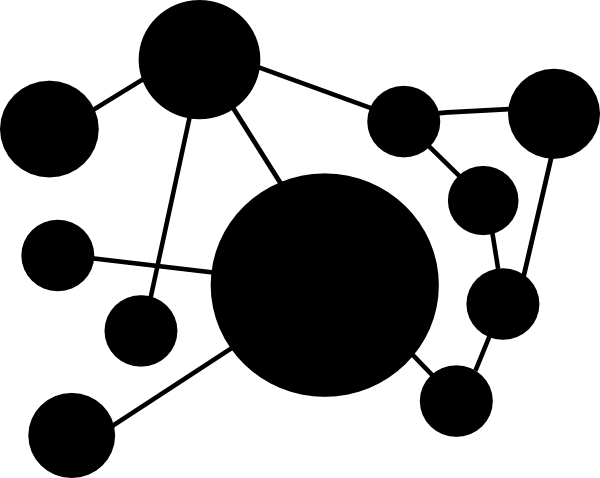
\includegraphics[width=50mm]{titelbild.png}} 
\publishers{
\includegraphics[width=100mm]{TH-Logo.jpg}}

%Zur Überscchrift machen
\maketitle

\pagenumbering{Roman}
%Verzeichnisse
\tableofcontents
\listoffigures
\listoftables
\listofformels
\chapter*{Abkürzungsverzeichnis}
\addcontentsline{toc}{chapter}{Abkürzungsverzeichnis}
\begin{acronym}[SEPSEP]
\acro{knn}[KNN]{Künstliches neuronales Netz}
\acro{dax}[DAX]{Deutscher Aktienindex}
\acro{gui}[GUI]{Graphical User Interface}
\end{acronym}  
 
%Eigentliche Text beginnt hier
\chapter{Einleitung} %Beide
 \pagenumbering{arabic}
\label{cha:Einleitung}
\section{Motivation}
\label{sec:Motivation}
Die Untersuchung und Extrapolation von Zeitreihen ist ein bedeutendes Thema in zahlreichen Gebieten. Typische Anwendungsbereiche sind zum Beispiel die Prognose von Wetterdaten, von Therapieverläufen in der  Medizin, von Arbeitslosenzahlen auf dem Arbeitsmarkt sowie von Börsenkursen. Um eine Zeitreihe möglichst genau zu extrapolieren, wird auf mehreren Hilfsmitteln zurückgegriffen. Einer dieser Hilfsmittel können künstliche neuronale Netze sein. 

Bei künstlichen neuronalen Netzen handelt es sich um Netzwerke mit künstlichen Neuronen als Knoten, die mittels gerichtete Verbindungen Eingaben einlesen, weiterverarbeiten und die daraus resultierenden Ergebnisse an weitere Neuronen weiterleiten oder als Ergebnis ausgeben. Bei der Terminologie von künstlichen neuronalen Netzen wird bewusst auf Begriffen der Biologie zurückgegriffen, da künstliche neuronale Netze das biologische Gehirn als Vorbild nutzen und dessen Herangehensweise auf analoger Weise umzusetzen zu versuchen. Man nennt das Verfahren dieser Netze aus diesem Grunde auch \textit{naturanaloge Verfahren}.

Warum sind diese Netze nun so interessant für Prognosen? Das Erstellen von zum Beispiel Börsenprognosen basiert in der Regel auf Auswertungen von Informationen verschiedenster Quellen. Die Art von Auswertungen, wie Börsenexperten sie vornehmen, ist weder vollständig formalisierbar noch besonders exakt, da uneinheitlich und in weiten Zügen intuitiv. Besonders schwer ist hier das Ermitteln von \textit{nichtlinearen Zusammenhängen}. Ein \ac{knn} ist jedoch in der Lage, diese Zusammenhänge zu finden  und diese objektiv und vorurteilsfrei zu bewerten. Somit sind künstliche neuronale Netze prinzipiell in der Lage, jedes beliebige Muster in jedem beliebigen Markt zu erkennen - auch solche, die noch nie zuvor von irgend jemand entdeckt wurden.

Ob und wie gut \ac{knn} zur Prognose geeignet sind, ist pauschal nicht zu beantworten. In manchen Gebieten mag die Prognosefähigkeit durchaus ausreichen. Je höher die geforderte Genauigkeit jedoch wird, desto diskutabler wird ein Einsatz von \ac{knn}. Eine typische Grauzone ist hier die Prognose von Börsenkursen. Während Befürworter auf die Eigenschaft von \ac{knn} hinweisen, nichtlineare Muster zu erkennen und entsprechend zu behandeln, argumentieren Kritiker, dass ein System, das dem menschlichen Lernen nachempfunden wurde, die gleichen Fehler machen wird wie der Mensch. Generell ist jedoch zu sagen, das die Prognosequalität von künstlichen \ac{knn} über die Jahre stets angestiegen ist.


\section{Ziel und Aufbau dieser Arbeit}
\label{sec:Ziel}
Als Ziel dieser Seminararbeit wird versucht ein \ac{knn} zu erschaffen, das prinzipiell in der Lage ist, den Börsenkurs des Deutschen Aktienindex (\acs{dax}) vorherzusagen. Der Fokus dieser Arbeit liegt hierbei nicht auf möglichst genaue Prognosen, sondern auf das Erlangen eines Grundverständnisses über die Funktionsweise von \ac{knn}. Trotzdem ist ein bestimmtes Maß an Genauigkeit ein wichtiges Kriterium, das es zu berücksichtigen gilt. Dieses \ac{knn} soll anschließend in einer Anwendung überführt werden, die die Prognosen und die dazugehörige Prognosequalität visualisiert.

Zur Erlangung des Ziels der Seminararbeit müssen mehrere Teilschritte durchgeführt werden. Das Vorgehen während dieser Seminararbeit wird im folgenden Diagramm visualisiert:
 
\begin{figure}[htbp]
\centering
		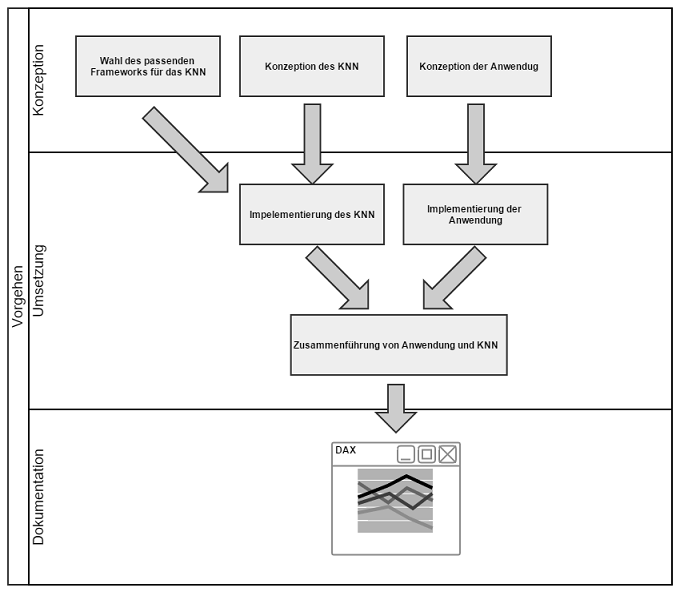
\includegraphics[width=0.95\textwidth]{Vorgehensdiagramm.PNG}
	\caption{Vorgehensdiagramm}
	\label{fig:Vorgehensdiagramm}
\end{figure}


Zunächst wird mit einer Konzeptionsphase begonnen. in dieser wird zunächst eine fachliche Konzeption der Anwendung erstellt, in der die Funktionalitäten der Anwendungen genau spezifiziert werden. Abgerundet wird diese Fachkonzeption durch ein Mockup. Nachdem die Konzeption der Anwendung abgeschlossen wurde, wird das benötigte \ac{knn} für diese Anwendung konzeptioniert. Dabei ist zu ermitteln, welches \ac{knn} hinsichtlich Typ, Topologie und Lernverfahren am Besten für die Prognose des \ac{dax} geeignet ist. Zur Erstellung von \ac{knn} stehen mehrere Frameworks zur Verfügung, drei dieser Frameworks werden genauer analysiert und im Anschluss das für diese Seminararbeit geeignetste Framework ausgewählt.

Nachdem die Konzeptionsphase abgeschlossen ist, wird mit der Umsetzung der Anwendung begonnen. Die Umsetzungsphase besteht im Wesentlichen aus drei Teilen. Zu einen aus der Implementierung des \ac{knn} und der Anwendung und zum anderen aus der Zusammenführung der beiden Elemente. 

Nachdem die Anwendung entsprechen umgesetzt wurde, wird diese beschrieben. Konkret werden hierbei die einzelnen Elemente des \ac{gui} sowie die technische Architektur der Anwendung beschrieben.

 
\chapter{Konzeption}
\label{cha:Konzeption}
\section{Fachliche Konzeption der Anwendung} %Benedikt
\label{sec:faco}
\subsection{Beschreibung der Anwendung}
\label{subsec:beaw}
\subsection{Mockup der Anwendung}
\label{subsec:moaw}
\begin{figure}[htbp]
\centering
		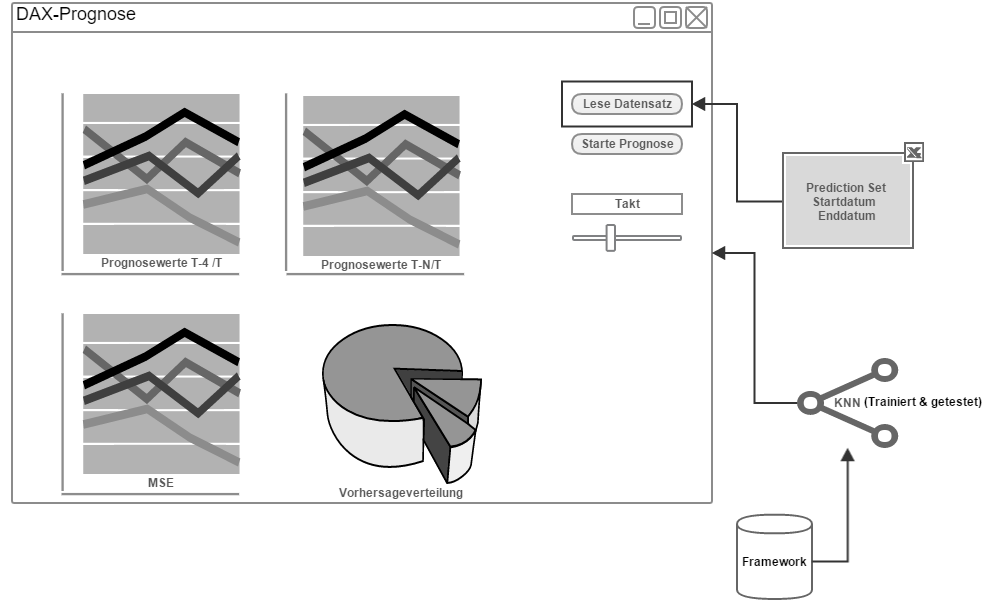
\includegraphics[width=0.95\textwidth]{mockup.PNG}
	\caption{Mockup der Anwendung}
	\label{fig:Mockup der Anwendung}
\end{figure}


\section{Konzeption des künstlichen neuronalen Netzes} %Sebastian
\subsection{Typ des künstlichen neuronalen Netzes} %Sebastian
\subsection{Grundlegende Topologie des künstlichen neuronalen Netzes} %Sebastian

\begin{figure}[H]
\centering
		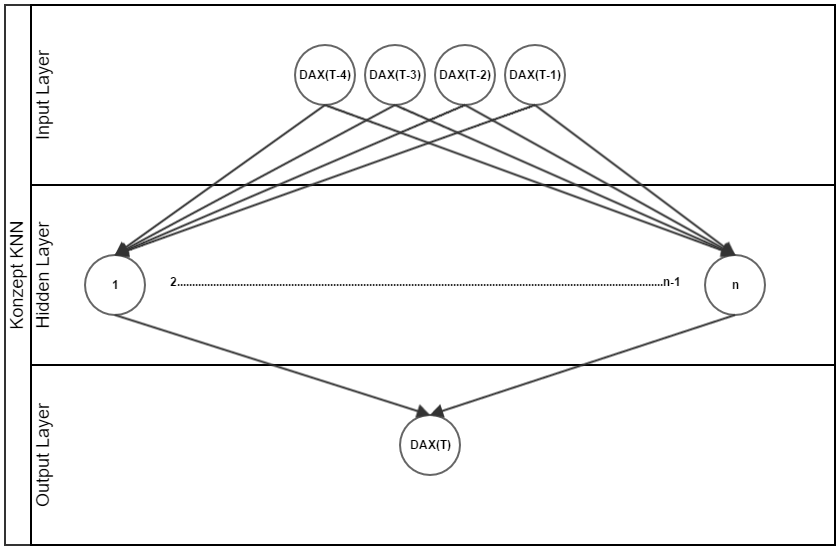
\includegraphics[width=0.95\textwidth]{KonzeptKNN.PNG}
	\caption{Grundlegendes Konzept des KNN}
	\label{fig:Grundlegendes Konzept des KNN}
\end{figure}

\subsection{Lernverfahren des künstlichen neuronalen Netzes} %Sebastian
\section{Beschreibung von Frameworks} %Benedikt
\subsection{SNNS} %Benedikt
\subsection{JavaNNS}  %Benedikt
\subsection{Neuroph} %Benedikt
\section{Wahl des geeignetsten Frameworks} %Benedikt
\chapter{Umsetzung} %Beide
\section{Erstellung des künstlichen neuronalen Netzes} %Sebastian

beschreibung folgende 3 abschnitte sukzessive
normalisierungsfunktion
beispieldatensatz (training / test)
verteilung(training/test)
menge(training/test)
Anzahl Durchläuge: 100k
Lernrate 0.5


\subsection{Ermittlung der genauen Topologie} %Sebastian
In der Literatur wird dabei oft auf die folgende Gleichung zur Ermittlung der optimalen  Menge an Neuronen der versteckten Schicht angegeben:

\begin{equation}\formelentry{Optimale Anzahl Neuronen in der versteckten Schicht}
  N_h = \frac{N_d}{10*(N_i+N_o)}
\end{equation}


\begin{figure}[htbp]
\centering
		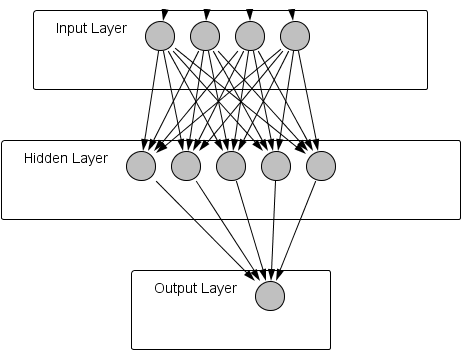
\includegraphics[width=0.75\textwidth]{4-5-1.PNG}
	\caption{KNN nach 4-05-1 Muster}
	\label{fig:KNN nach 4-05-1 Muster}
\end{figure}


\begin{figure}[H]
\centering
		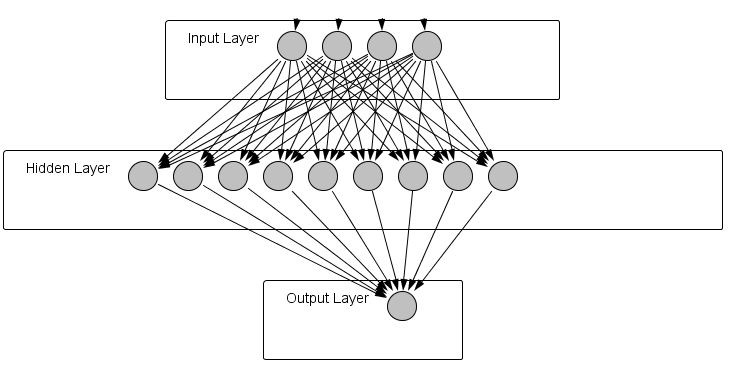
\includegraphics[width=0.75\textwidth]{4-9-1.PNG}
	\caption{KNN nach 4-09-1 Muster}
	\label{fig:KNN nach 4-09-1 Muster}
\end{figure}



\begin{figure}[htbp]
\centering
		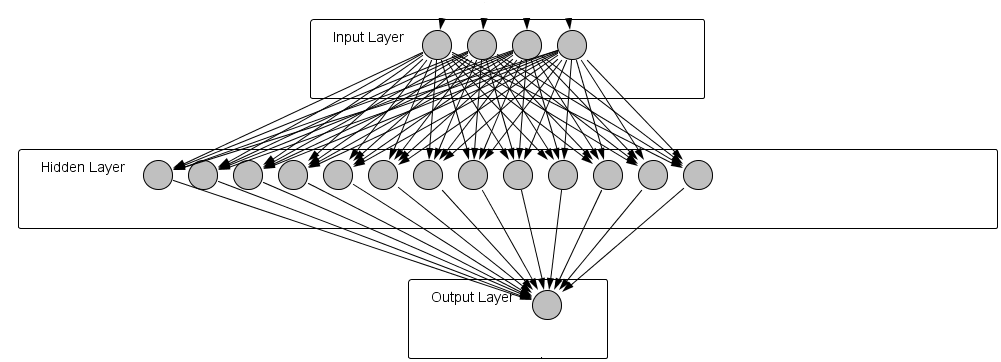
\includegraphics[width=0.75\textwidth]{4-13-1.PNG}
	\caption{KNN nach 4-13-1 Muster}
	\label{fig:KNN nach 4-13-1 Muster}
\end{figure}


\begin{table}
  \centering
  \begin{tabular}{|c|c|}
  \hline 
  \rule[0ex]{0pt}{2.5ex} Topologie & Mean Squared Error \\ 
  \hline 
  \rule[0ex]{0pt}{2.5ex} 4-05-1 & 0.000 \\ 
  \hline 
  \rule[0ex]{0pt}{2.5ex} 4-09-1 & 0.000 \\ 
  \hline 
  \rule[0ex]{0pt}{2.5ex} 4-13-1 & 0.000 \\ 
  \hline 
  \end{tabular} 
  \caption{Jeweilige Topologien \& korrespondierende MSE}
  \label{tab:myfirsttable}
\end{table}


\subsection{Ermittlung der Transferfunktion} %Sebastian

Sigmoide Funktion:

\begin{equation}\formelentry{Sigmoide Funktion}
f(x)= \frac{1}{1+e^{-cx}}
\end{equation}

\begin{figure}[htbp]
\centering
		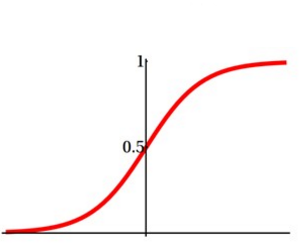
\includegraphics[width=0.5\textwidth]{Sigmoid.PNG}
	\caption{Sigmoide Funktion}
	\label{fig:Sigmoide Funktion}
\end{figure}

Tangens Hyperbolicus:

\begin{equation}\formelentry{Tanh Funktion}
f(x)= tanh(x)
\end{equation}

\begin{figure}[htbp]
\centering
		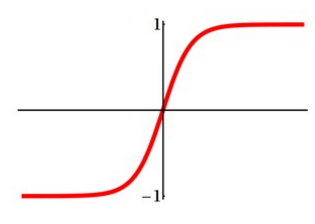
\includegraphics[width=0.5\textwidth]{tanh.PNG}
	\caption{Tangens Hyperbolicus Funktion}
	\label{fig:Tangens Hyperbolicus Funktion}
\end{figure}

\begin{table}
  \centering
  \begin{tabular}{|c|c|}
  \hline 
  \rule[0ex]{0pt}{2.5ex} Transferfunktion & Mean Squared Error \\ 
  \hline 
  \rule[0ex]{0pt}{2.5ex} 4-05-1 & 0.000 \\ 
  \hline 
  \rule[0ex]{0pt}{2.5ex} 4-09-1 & 0.000 \\ 
  \hline 
  \rule[0ex]{0pt}{2.5ex} 4-13-1 & 0.000 \\ 
  \hline 
  \end{tabular} 
  \caption{Jeweilige Transferfunktionen \& korrespondierende MSE}
  \label{tab:tab2}
\end{table}

\subsection{Ermittlung der Lernregel und Lernrate} %Sebastian

\begin{table}[H]
  \centering
  \begin{tabular}{|c|c|c|}
  \hline 
  \rule[0ex]{0pt}{2.5ex} Lernregel & beste Lernrate & Mean Squared Error \\ 
  \hline 
  \rule[0ex]{0pt}{2.5ex} Backpropagation & 0.000 & 0.000 \\ 
  \hline 
  \rule[0ex]{0pt}{2.5ex} Momentum Backpropagation & 0.000 & 0.000\\ 
  \hline 
  \rule[0ex]{0pt}{2.5ex} Resilient Propagation & 0.000 & 0.000 \\ 
  \hline 
  \end{tabular} 
  \caption{Jeweilige Lernregeln und beste Lernraten \& korrespondierende MSE}
  \label{tab:tab3}
\end{table}
\section{Das erstellte künstliche neuronale Netz}
\section{Implementierung der Anwendung} %Benedikt
\section{Zusammenführung des Netzes mit der Anwendung}


\chapter{Beschreibung der Anwendung} %Benedikt
\section{Elemente der GUI} %Beide
\section{Architektur der Anwendung} %Benedikt

\chapter{Fazit} %Beide
\label{cha:Fazit}
Das prognostizieren von Börsenkursen mittels künstlichen neuronalen Netzen ist möglich.

%Literaturverzeichnis anzeigen
\bibliography{Literatur}

\end{document}